\documentclass{beamer}
\usetheme{Berlin}
\usepackage{graphicx}
\usepackage[UKenglish]{isodate}
\usepackage{tikz}

\graphicspath{{./images/}}
\beamertemplatenavigationsymbolsempty

\title{Processor Simulator}
\author{George Herbert}
% \institute[University of Bristol, Bristol, U.K.]{University of Bristol\\Bristol, U.K.}
\date{\today}

\begin{document}

\begin{frame}
    \titlepage
\end{frame}

\section{Architecture}
\begin{frame}{High-Level Architecture Diagram}
    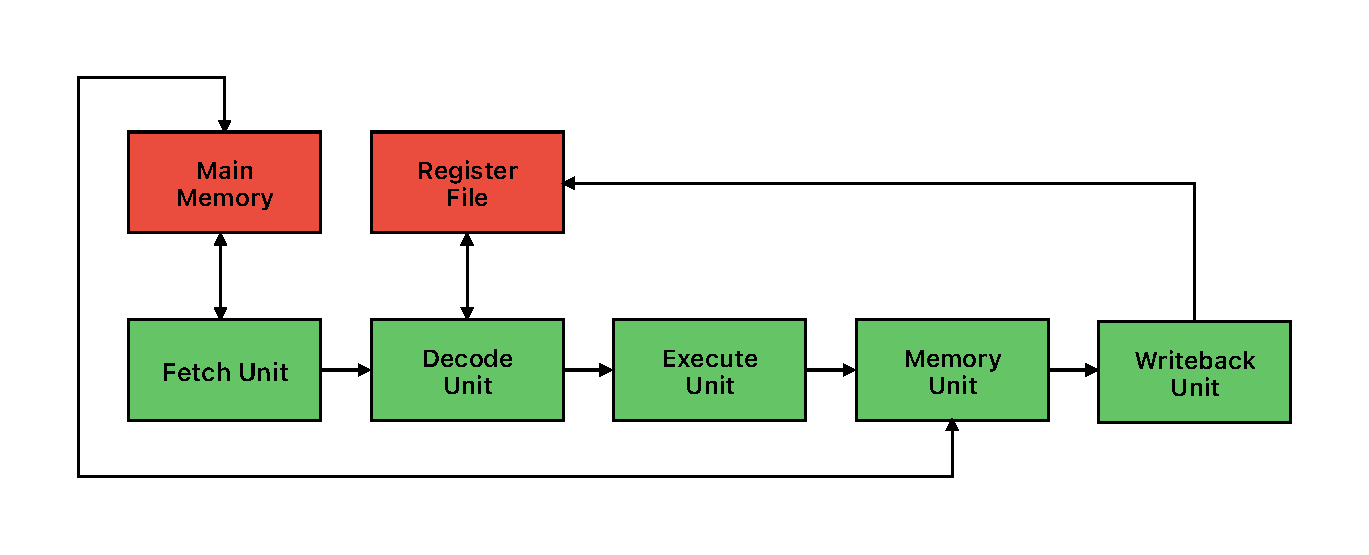
\includegraphics[width = \textwidth]{architecture.pdf}
\end{frame}

\begin{frame}{Features}
    \begin{itemize}
        \item Non-pipelined and scalar
        \item Five-stage cycle: fetch, decode, execute, memory, writeback
        \item Implements the RV32I base integer instruction set, except for the FENCE, ECALL, and EBREAK instructions
        \item Operation of each unit is dictated by control signals produced by the decode unit
    \end{itemize}
\end{frame}

\section{Benchmark Kernels}
\begin{frame}{Euclidean}
    
\end{frame}

\end{document}
